\documentclass[a4paper,14pt,russian]{article}
\usepackage{./coursework}
\usepackage{titlesec}
\usepackage[export]{adjustbox}
\usepackage{lastpage}
\newcommand{\caphedre}{ВТ}
\newcommand{\theme}{Проектирование цифровых узлов на микросхемах программируемой логики}
\newcommand{\groupnumber}{5305}
\newcommand{\studentname}{Билькис П.П.}
\newcommand{\teachername}{Буренева О.И.}
\newcommand{\discipline}{Узлы и устройства средств вычислительной техники}
\newcommand{\myyear}{2018}
\begin{document}

\begin{titlepage}

\thispagestyle{empty}

\centerline{МИНОБРНАУКИ РОССИИ}
\centerline{САНКТ-ПЕТЕРБУРГСКИЙ ГОСУДАРСТВЕННЫЙ}
\centerline{ЭЛЕКТРОТЕХНИЧЕСКИЙ УНИВЕРСИТЕТ}
\centerline{<<ЛЭТИ>> ИМ. В.И. УЛЬЯНОВА (ЛЕНИНА)}
\centerline{Кафедра \caphedre}

\vfill

\centerline{\large{\textsc{КУРСОВОЙ ПРОЕКТ}}}
\centerline{\large{по дисциплине <<\discipline>>}}
\centerline{\large{Тема: \theme}}

\vfill

Студент группы \groupnumber \hfill \studentname

Преподаватель \hfill \teachername

\vfill

\centerline{Санкт-Петербург}
\centerline{\myyear}
\clearpage
\end{titlepage}
\setcounter{page}{2}

\section*{Задание на курсовой проект}
Студент \studentname\\
Группа \groupnumber\\\\
Тема работы: \theme (многорежимный формирователь импульсных последовательностей) \\
Исходные данные:\\
Разработать принципиальную электрическую схему устройства, формирующего заданные последовательности импульсов. Входные сигналы поступают от ГТИ (генератор следует разработать). Выходные последовательности цикличны. Длина цикла N периодов тактирующих импульсов, на выходе должны формироваться импульсы с указанными в задании номерами и заданной скважинностью.
Содержание пояснительной записки:\\
«Аннотация», «Содержание», «Введение», ... ,«Заключение», «Приложения».
Предполагаемый объем пояснительной записки:\\
Не менее \pageref{LastPage}
Дата выдачи задания: 01.02.2018\\
Дата сдачи реферата: 01.06.2018\\
Дата защиты реферата: 01.06.2018\\

\vfill


Студент группы \groupnumber \hfill \studentname


Преподаватель \hfill \teachername


\clearpage

\selectlanguage{russian}
\begin{abstract}
  абстракт на русском
\end{abstract}


\selectlanguage{english}
\begin{abstract}
  abstract here
\end{abstract}

\clearpage

\selectlanguage{russian}
\tableofcontents
\clearpage

\section*{Введение}
\addcontentsline{toc}{section}{Введение}
введение
\clearpage

\section{Задание на проектирование узла}

\subsection{Общее задание}
Разработать принципиальную электрическую схему устройства, формирующего заданные последовательности импульсов. Входные сигналы поступают от ГТИ (генератор следует разработать). Выходные последовательности цикличны. Длина цикла N периодов тактирующих импульсов, на выходе должны формироваться импульсы с указанными в задании номерами и заданной скважинностью.
Распределитель рассматривается как ВУ процессорной системы, его адреса начинаются с адреса 0x30 и заканчиваются адресом 0x35.

\subsection{Вариант 1.4}
В таблице \ref{table:task} приведены параметры, уточняющие задание.
\begin{table}[h]
  \centering
  \begin{tabular}{|l|l|l|l|l|l|l|l|p{2cm}|l|}
    \hline
    Вариант & N &  \multicolumn{6}{|c|}{Номера импульсов} & Начальный \newline адрес & Скважинность \\ \cline{3-8}
            & & \multicolumn{6}{|c|}{Режимы} & & \\ \cline{3-8}
            & & 1 & 2 & 3 & 4 & 5 & 6 & & \\ \hline 
    1.4 & 22 & 3,8,11,20 & 2,4,12,21 & 5,10,15,16 & 8,9,13,17 & 1,6,11,19 & 1,2,7,9,18,22 & 0x30 & 8 \\ \hline
  \end{tabular}
  \caption{Параметры задания}
  \label{table:task}
\end{table}

\section{Сравнительный анализ предлагаемых вариантов}

\subsection{Реализация узла на основе счётчика и дешифратора}
Разрабатываемый в данном курсовом проекте узел состоит из нескольких логических частей: устройства управления (УУ), трехразрядного регистра режима и непосредственно формирователя импульсной последовательности. Структурная схема приведена на рис. \ref{fig:structure}.\\
Структурная схема многофункционального формирователя импульсной последовательности приведена на рис. \ref{fig:nodestructure}

\begin{figure}
  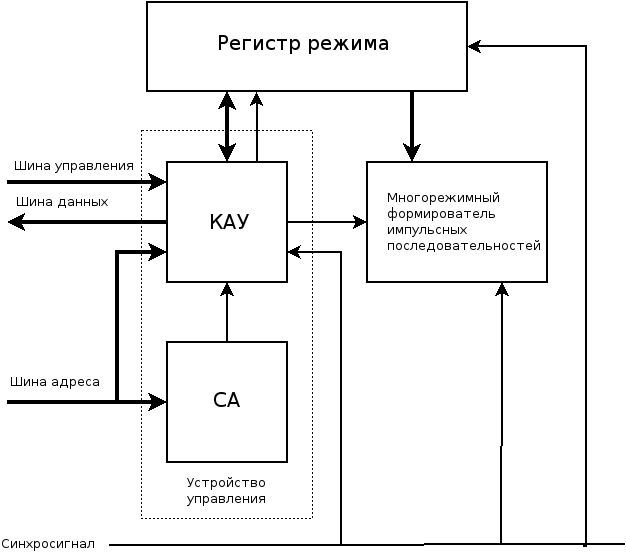
\includegraphics[scale=0.58]{./structure.png}
  \caption{Структура узла. СА - селектор адреса, КАУ - конечный автомат управления.}
  \label{fig:structure}
\end{figure}

\begin{figure}
  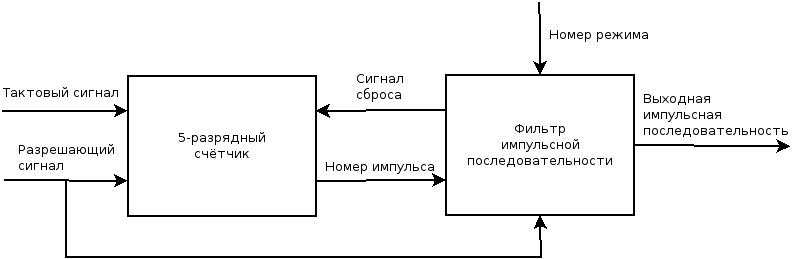
\includegraphics[scale=0.58]{./node-structure.png}
  \caption{Структура многофункционального формирователя импульсной последовательности}
  \label{fig:nodestructure}
\end{figure}

Для корректной работы устройства должны присутствовать:
\begin{itemize}
\item Шина данных (ШД)
\item Шина управления (ШУ)
\item Шина адреса (ША)
\item Тактирующий сигнал
\end{itemize}
\noindent Подробное описание интерфейса разрабатываемого устройства и протокол его работы представлены в разделе <<\nameref{sections:iface}>>



\subsection{Реализация узла на основе счётчика и двух мультиплексорах}
Задача узла заключается в формировании выходной импульсной последовательности из входной, выбирая только некоторые, в зависимости от режима, импульсы, с периодом в 22 импульса. Например, в первом режиме (3, 8, 11, 20) на выход подадутся (считая от единицы): 3-й, 8-й, 11-й, 20-й, (3+22)-й, (8+22)-й, (11+22)-й, (20+22)-й и т.д. импульсы.\\
Идея первого варианта узла заключается в следующем. По входному тактовому сигналу работает счётчик, который считает от 0 до 21, циклично. Счётчик формирует 5-разрядное число на выходе. Данные пять разрядов используются, чтобы выбрать один из 22-х выходов дешифратора. Выходы дешифратора объединены в шесть частично пересекающихся групп через элементы ИЛИ, в соответствии со вариантами режимов. Т.е., когда счётчик досчитывает до некоторого числа n (т.е. когда на вход приходит (n+1)-й импульс), элементы ИЛИ, в которые входит данное число, выдают логическую единицу, все остальные - логический ноль. Таким образом осуществляется фильтрация входного тактового сигнала в соответствии со всеми режимами, формируется шесть импульсных последовательностей. При помощи мультиплексора, по номеру режима, осуществляется коммутация одной из этих последовательностей на выход. Функциональная схема данного узла представлена на рис. \ref{fig:firstnode}.
\begin{figure}
  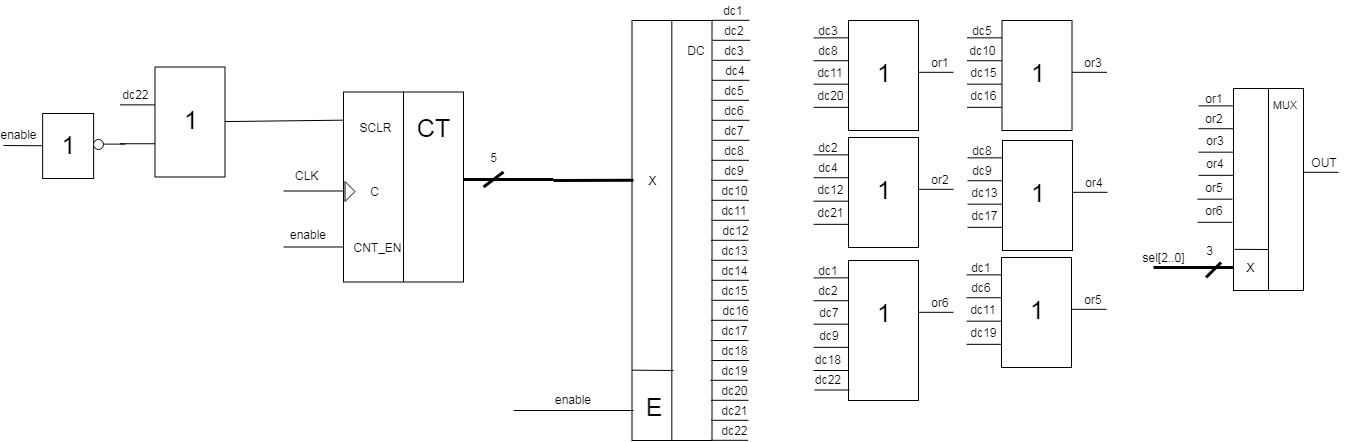
\includegraphics[scale=0.35]{./first-node.png}
  \caption{Функциональная схема многорежимного формирователя импульсной последовательности. Вариант 1.}
  \label{fig:firstnode}
\end{figure}

\subsection{Выбор оптимальной схемы}
Первая составляющая формирователя - счётчик - во втором варианте ничем не отличается от первого. 5-разрядный выход счётчика подаётся на мультиплексор, который коммутирует один из своих 22 входов на выход. На дешифратор подаётся номер режима, данный узёл выставляет единицу на один из своих шести выходов в соответствии с режимом работы формирователя. Идея заключается в следующем: каждый из коммутируемых входов мультиплексора представляет собой один из 22-х импульсов в периодичной импульсной последовательности. Требуется установить в единицу только те импульсы, который должны присутствовать в данном режиме, остальные следует держать на нуле. Для достижения данной цели, выход из дешифратора, который соответствует определённому режиму, подаётся на те входы мультиплексора, которые соответствуют единичным импульсам в текущем режиме. Остальные импульсы, по природе работы дешифратора, будут нулями. Функциональная схема второго варианта представлена на рис. \ref{fig:secondnode}.
\begin{figure}
  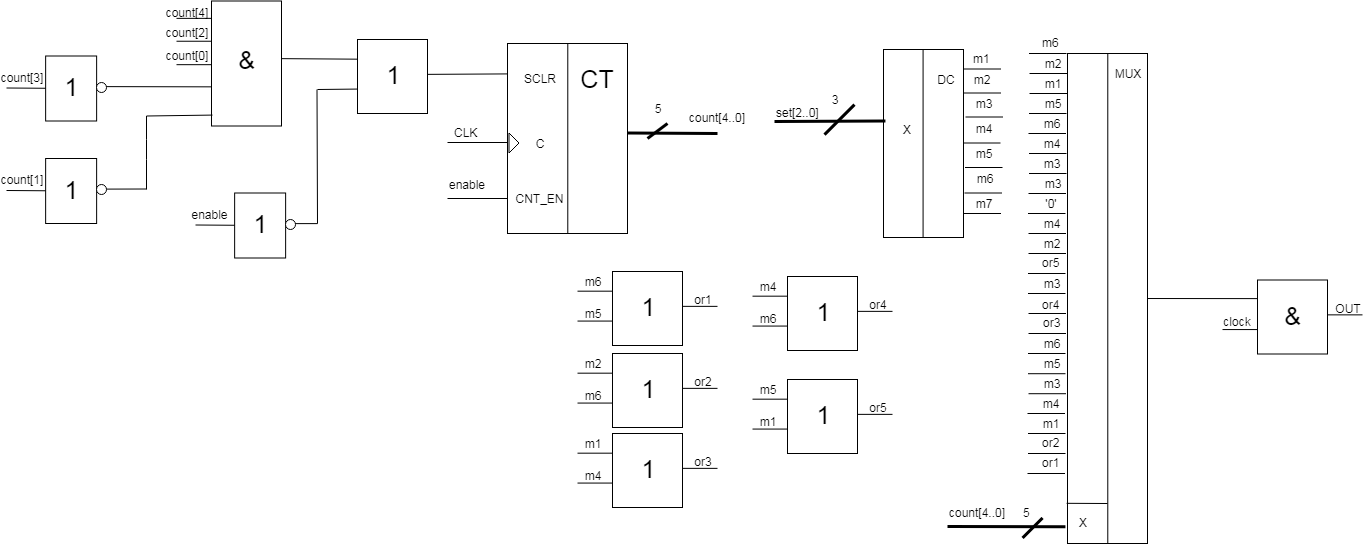
\includegraphics[scale=0.35]{./second-node.png}
  \caption{Функциональная схема многорежимного формирователя импульсной последовательности. Вариант 2.}
  \label{fig:secondnode}
\end{figure}

\section{Описание основных элементов библиотеки сапр Quartus II и стандартных микросхем, необходимых для реализации узла}

\subsection{Список использованных элементов}
Для реализации узла были использованы следующие примитивы из библиотеки САПР Quartus II:
\begin{itemize}
\item элемент <<НЕ>>
\item элемент <<6-И>>
\item элемент <<2-И>>
\item элемент <<2-ИЛИ>>
\end{itemize}
Из настраиваемых компонентов библиотеки САПР Quartus II использовались следующие:
\begin{description}
\item[5-разрядный счётчик] с выходом для синхроного сброса (sclr) и выходом для остановки/начала счёта (cnt\_en). Представлен на рисунке \ref{fig:ct}
  
\item[8-разрядный дешифратор (используются только первые шесть разрядов)] см. рис. \ref{fig:dc}
\item[32-разрядный мультиплексер (используются только первые 22 разряда)] см. рис. \ref{fig:mux}
\end{description}

\begin{figure}
  \begin{center}
    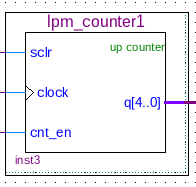
\includegraphics[scale=1]{./ct.png}
    \caption{5-разрядный счётчик в САПР Quartus II.}
    \label{fig:ct}
  \end{center}
\end{figure}

\begin{figure}
  \begin{center}
    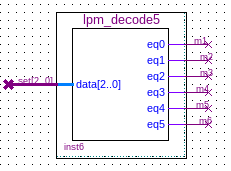
\includegraphics[scale=1]{./dc.png}
    \caption{8-разрядный дешифратор (используются только первые шесть разрядов) в САПР Quartus II.}
    \label{fig:dc}
  \end{center}
\end{figure}

\begin{figure}
  \begin{center}
    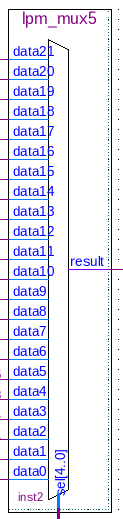
\includegraphics[scale=0.6]{./mux.png}
    \caption{32-разрядный мультиплексер (используются только первые 22 разряда) в САПР Quartus II.}
    \label{fig:mux}
  \end{center}
\end{figure}

\subsection{Характеристики используемой интегральной схемы}
Данный узёл разрабатывается с упором на его реализацию с использованием ПЛИС Cyclone II EP2C5Q208C8. Основные параметры данной ПЛИС приведены в таблице \ref{table:fpga}. Выбор данной ПЛИС обусловлен в первую очередь её доступностью, а так же близким знакомством автора с ПЛИС данной серии, полученным в ходе освоения курса <<Узлы и устройства ЭВМ>>.

\begin{table}[h]
  \centering
  \begin{tabular}{|l|l|}
    \hline
    Семейство ПЛИС & Cyclone II \\ \hline
    Количество логических блоков &  4608 \\ \hline
    Корпус & 208-Pin PQFP \\ \hline
    Полное количество RAM & 1.1 Mbytes \\ \hline
    Количество I/O & 142 \\ \hline
    Напряжение питания I/O  & 1.5, 1.8, 2.5, 3.3 V \\ \hline
    Максимальная рабочая частота & 260 MHz \\ \hline
  \end{tabular}
  \caption{Параметры ПЛИС Cyclone II EP2C5Q208C8}
  \label{table:fpga}
\end{table}

\section{Процесс синтеза первого варианта схемы средствами САПР Quartus II}
Согласно структурной схеме многорежимного формирователя импульсной последовательности, данный элемент состоит из двух основных блоков:
\begin{itemize}
\item 5-разрядный счётчик
\item Фильтр импульсной последовательности
\end{itemize}

5-разрядный счётчик представляет собой готовый настраиваемый компонент САПР Quartus II - lpm\_counter. Фильтр импульсной последовательности реализуется в соответствии с функциональной схемой (см. рис. \ref{fig:secondnode}). Для реализации фильтра используются следующие элементы САПР Quartus II:
\begin{itemize}
\item элемент <<НЕ>>
\item элемент <<6-И>>
\item элемент <<2-И>>
\item элемент <<2-ИЛИ>>
\item 8-разрядный дешифратор (используются только первые шесть разрядов, см. рис. \ref{fig:dc}
\item 32-разрядный мультиплексер (используются только первые 22 разряда, см. рис. \ref{fig:mux}
\end{itemize}

\noindent Соединение элементов производится по функциональной схеме, представленной на рис. \ref{fig:secondnode}. Описание работы данной схемы представлено в разделе <<\nameref{sections:secondnode}>>.\\
Итоговая схема в САПР Quartus II представлена на рис. \ref{fig:finalscheme}. На рис. \ref{fig:compile} представлены результаты компиляции, на рис. \ref{fig:freq} оценка максимальной частоты работы устройства.

\begin{figure}
  \begin{center}
    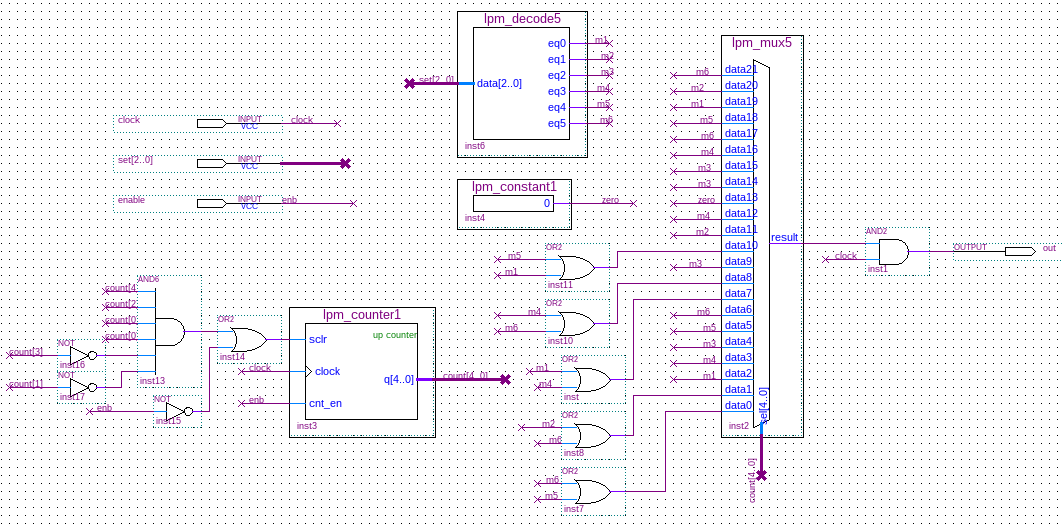
\includegraphics[scale=0.65]{./final-scheme.png}
    \caption{Итоговая схема в САПР Quartus II.}
    \label{fig:finalscheme}
  \end{center}
\end{figure}


\begin{figure}
  \begin{center}
    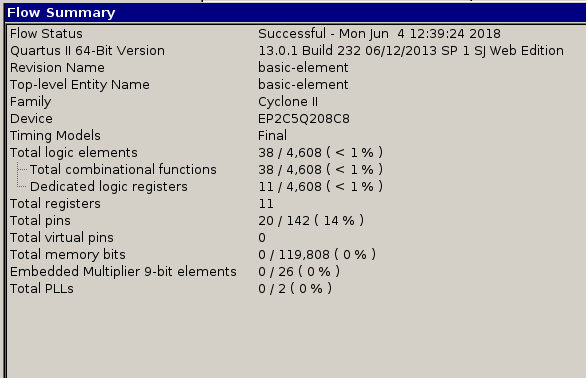
\includegraphics[scale=0.65]{./compile.png}
    \caption{Результаты компилирования в САПР Quartus II.}
    \label{fig:compile}
  \end{center}
\end{figure}

\begin{figure}
  \begin{center}
    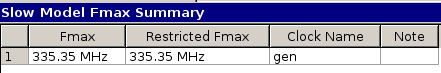
\includegraphics[scale=0.65]{./freq.png}
    \caption{Оценка максимальной частоты работы устройства в САПР Quartus II.}
    \label{fig:freq}
  \end{center}
\end{figure}

\section{Разработка интерфейса сопряжения схемы узла с процессорной системой}
Устройство управления представляет собой интерфейс узла, через который осуществляется всё взаимодействие с внешним миром. УУ состоит из селектора адреса (CА) и конечного автомата управления (КАУ). Селектор адреса (СА) читает шину адреса (ША) и при поступлении адреса из нужного диапазона (0x30-0x35) формирует сигнал разрешения. При разрешении от СА, КАУ может работать. КАУ читает шину управления (ШУ) - 2 разряда - и реагирует на следующие сигналы от неё:
\begin{description}
\item[01] Сигнал START. УУ запускается, считывает режим работы из адреса в регистр режима и подаёт разрешающий сигнал на формирователь импульсной последовательности.
\item[10] Сигнал READ. Реакция на этот сигнал будет только при условии, что ранее подавался сигнал START, т.е. УУ запущено. При поступлении данного сигнала, УУ считывает три разряда из регистра режима и подаёт их на шину данных.
\item[11] Сигнал STOP. Реакция на этот сигнал будет только при условии, что ранее подавался сигнал START, т.е. УУ запущено. При поступлении данного сигнала, УУ перестаёт подавать разрешающий сигнал на формирователь импульсной последовательности и подаёт сигнал синхронного сброса на регистр режима. После этого УУ считается выключенным.
\end{description}

Режим работы формирователя импульсной последовательности передаётся в младших трёх битах 8-битного адреса, по ША, как часть адреса. В таблице \ref{table:modes} приведено соответствие между адресами и выходными импульсными последовательностями.

\begin{table}[h]
  \centering
  \begin{tabular}{|l|l|l|}
    \hline
    Адрес & Номер режима & Выходная последовательность импульсов \\ \hline
    0x30 & 1 & 3, 8, 11, 20 \\ \hline
    0x31 & 2 & 2, 4, 12, 21 \\ \hline
    0x32 & 3 & 5, 10, 15, 16 \\ \hline
    0x33 & 4 & 8, 9, 13, 17 \\ \hline
    0x34 & 5 & 1, 6, 11, 19 \\ \hline
    0x35 & 6 & 1, 2, 7, 9, 18, 22 \\ \hline
  \end{tabular}
  \caption{Соответствие адресов различным режимам}
  \label{table:modes}
\end{table}

Селектор адреса представляет собой простой элемент И, входами которого являются разряды адреса. Функциональная схема селектора адреса приведена на рис. \ref{fig:selector}.

\begin{figure}
  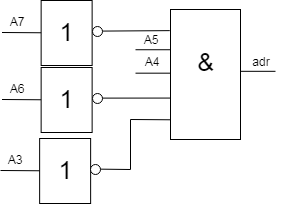
\includegraphics[scale=1]{./selector.png}
  \caption{Функциональная схема селектора адреса}
  \label{fig:selector}
\end{figure}

Конечный автомат управления представляет из себя конечный автомат Мура, генерирующий управляющие сигналы и коммутирующий потоки данных. Автомат описан таблицей \ref{table:auto}. Функциональная схема конечного автомата управления приведена на рис. \ref{fig:fca}.

\begin{table}[h]
  \centering
  \begin{tabular}{|c|c|c|c|c|c|c|}
    \hline
    \multicolumn{3}{|c|}{Состояние}  &  Условие перехода & \multicolumn{3}{|c|}{Переход в} \\ \cline{1-3} \cline{5-7}
    Q3 & Q1 & Q0 & & Q3 & Q1 & Q0 \\ \hline
    0  & 0 & 0 & adr \& start & 0 & 0 & 1\\ \cline{4-7}
                                     &  &  &  \textoverline{adr \& start} & 0 & 0 & 0 \\ \hline
    0 & 0 & 1 & 1 & 0 & 1 & 0 \\ \hline
    0 & 1 & 0 & adr \& stop  & 1 & 0 & 0 \\ \cline{4-7}
                                     &  &  & adr \& rd & 0 & 1 & 1 \\ \cline{4-7}
                                     &  &  &  \textoverline{adr \& stop}  & 0 & 1 & 0 \\ \cline{4-7}
                                     &  &  &  \textoverline{adr \& rd} & 0 & 1 & 0 \\ \hline
    1 & 0 & 0 & 1 & 0 & 0 & 0 \\ \hline
    0 & 1 & 1 & 1 & 0 & 1 & 0 \\ \hline
  \end{tabular}
  \caption{Структурная таблица конечного автомата}
  \label{table:auto}
\end{table}

\begin{figure}
  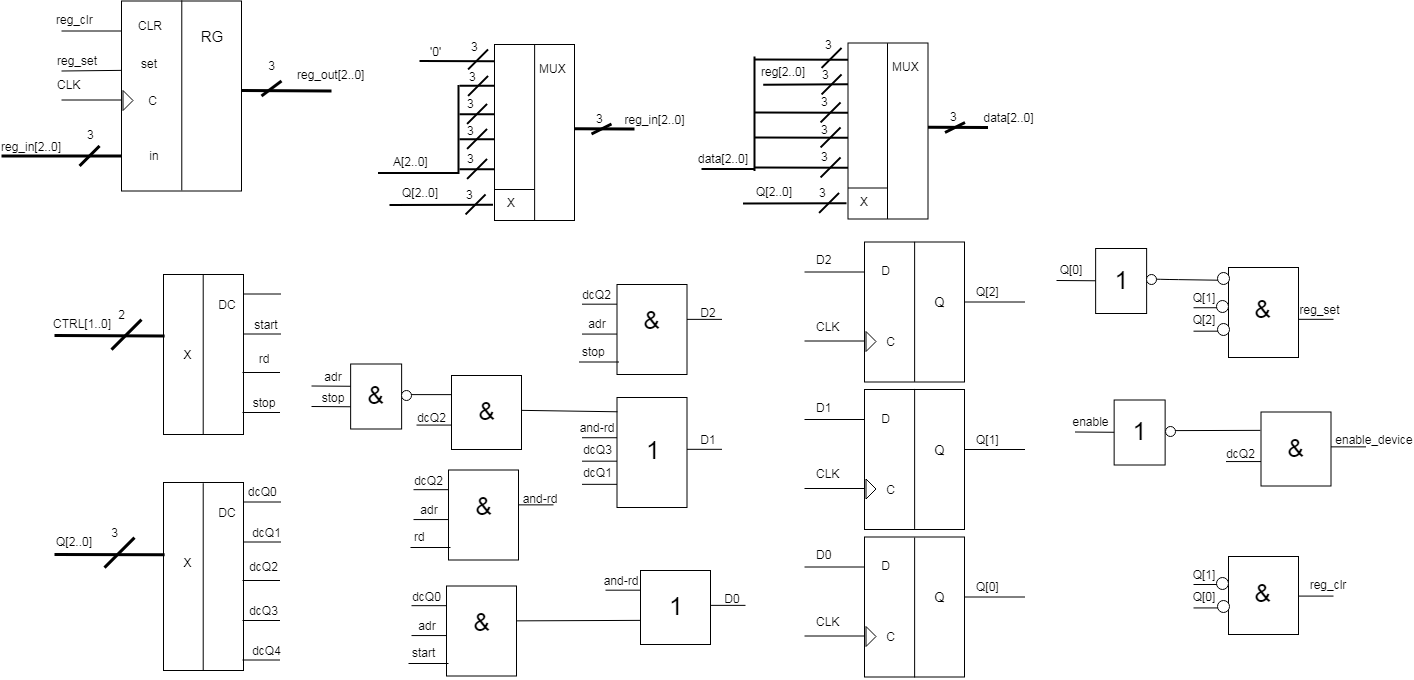
\includegraphics[scale=0.35]{./FCA.png}
  \caption{Функциональная схема }
  \label{fig:fca}
\end{figure}

\section{Описание функционирования узла с использованием необходимых временных диаграмм}
\subsection{Описание функцонирования узла}
Данное устройтво функционирует следующим образом.
\subsection{Функциональное моделирование}
На рисунке \ref{fig:funcmodel} представлены результаты функционального моделирования. На временной диаграмме продемонстрирована нормальная работа устройства: включение, работа, чтение режима, выключение, включение с другим адресом и т.д. Продемонстрированы разные режимы работы и переключения между ними.
\begin{figure}
  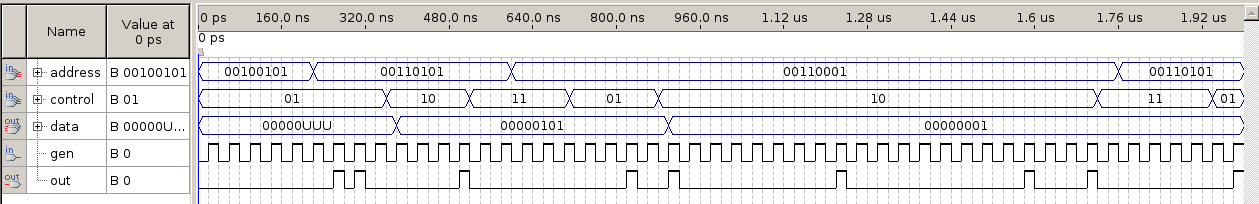
\includegraphics[scale=0.5]{./func-switching.png}
  \caption{Функциональное моделирование узла.}
  \label{fig:funcmodel}
\end{figure}

\section{Полная принципиальная электрическая схема разработанного узла}
\subsection{Разработка схемы питания}
\input{./sections/sc7-1.tex}
\subsection{Внешние подключения}
\input{./sections/sc7-2.tex}
\subsection{Схема узла}
\input{./sections/sc7-3.tex}
\section*{Заключение}
\addcontentsline{toc}{section}{Заключение}
В процессе курсового проекта

\renewcommand\refname{Список использованных источников}
\nocite{*}
\bibliographystyle{./utf8gost705u}
\bibliography{biblio}
\clearpage
\appendix

\end{document}
